\newpage
\section{Praktikum 1: Crawling, Linkextraktion und Content-Extraktion}

\subsection{DarmstadtSpider Analyse}

\subsubsection*{Top-Level Domains}

\begin{center}
	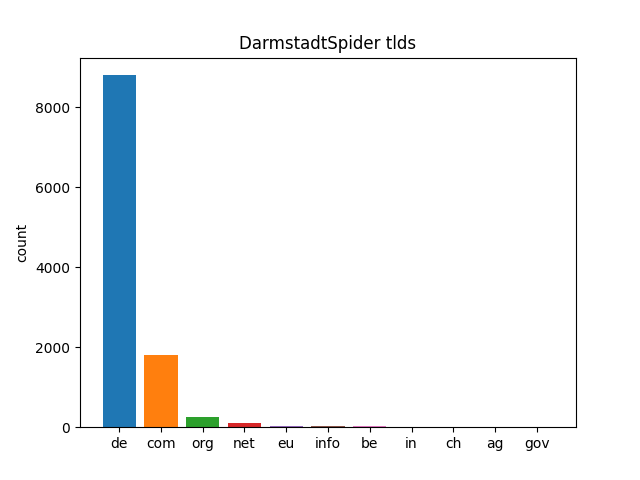
\includegraphics[width=0.6\textwidth]{images/DarmstadtSpiderTLDs.png}
\end{center}

\noindent Die mit Abstand häufigste Top-Level Domain (TLD) der verlinkten Webseiten ist 'de', was bei einer deutschen Webseite zu erwarten war. Am Zweithäufigsten mit etwa einem viertel dessen Häufigkeit steht 'com', was ebenfalls nicht verwunderlich ist, da diese TLD international, insbesondere in der westlichen Welt, am meisten vertreten ist.

\subsubsection*{Links}

Folgende ausgehende URLs, welche von mehreren Webseiten-Bereichen verlinkt wurden, sind uns besonders aufgefallen:

{\color{MidnightBlue}
\begin{lstlisting}
aka55plus.de
darmstadt.de/leben-in-darmstadt/soziales-und-gesellschaft/seniorinnen-und-senioren/
darmstadt.de/leben-in-darmstadt/bildung/aus-und-weiterbildung/
\end{lstlisting}}

\noindent$\Rightarrow$ Akademie 55plus Darmstadt e.V. (Aka 55plus) ist ein Verein für Bildung für Menschen ab dem 55. Lebensjahr. Somit passen die Bereiche \texttt{soziales-und-gesellschaft/seniorinnen-und-senioren} und \texttt{bildung/aus-und-weiterbildung} sehr gut.

{\color{MidnightBlue}
\begin{lstlisting}
cbf-da.de
darmstadt.de/leben-in-darmstadt/soziales-und-gesellschaft/menschen-mit-behinderung/
darmstadt.de/leben-in-darmstadt/mobilitaet-und-verkehr/barrierefrei/
\end{lstlisting}}

\noindent$\Rightarrow$ Club Behinderter und ihrer Freunde in Darmstadt und Umgebung e.V. (CBF) setzt sich für Menschen mit Behinderung ein. Auch hier passen die Bereiche \texttt{soziales-und-gesellschaft/menschen-mit-behinderung} und \texttt{mobilitaet-und-verkehr/barrierefrei} sehr gut.

{\color{MidnightBlue}
\begin{lstlisting}
gesetze-im-internet.de
darmstadt.de/leben-in-darmstadt/soziales-und-gesellschaft/frauen/aufgaben-und-ziele/
darmstadt.de/leben-in-darmstadt/umwelt/laerm/fluglaerm-in-darmstadt/laermschutzbereich-flughafen-frankfurt/
darmstadt.de/leben-in-darmstadt/soziales-und-gesellschaft/frauen/gleichstellungspolitik-in-der-stadtverwaltung/
darmstadt.de/leben-in-darmstadt/soziales-und-gesellschaft/frauen/gewaltschutz/
darmstadt.de/leben-in-darmstadt/mobilitaet-und-verkehr/radfahren-in-darmstadt/regeln-und-wissenswertes/
\end{lstlisting}}

\noindent$\Rightarrow$ All diese Bereiche, egal ob es um Frauenrechte, Fluglärm oder Radfahren geht, verweisen auf rechtliche Informationen auf der Webseite gesetze-im-internet.de des Bundesministeriums der Justiz und des Bundesamtes für Justiz.

\subsubsection*{Weitere Analyse}

Als weitere Analyse entschieden wir uns für eine Graphrepräsentation mittels \texttt{networkx} und \texttt{pyvis}.

\begin{center}
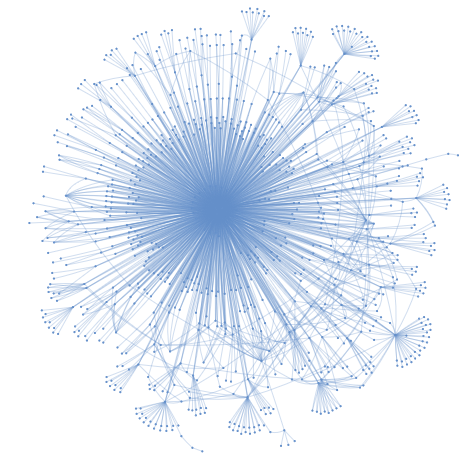
\includegraphics[width=0.6\textwidth]{images/DarmstadtSpiderGraph.png}
\end{center}

\noindent Bei genauerer Betrachtung zeigte uns diese Darstellung die eben gelisteten Informationen, konnten dann aber auch weiter verfolgt werden, um zum Beispiel von \texttt{gesetze-im-internet.de} über \\\texttt{darmstadt.de/leben-in-darmstadt/soziales-und-gesellschaft/frauen/aufgaben-und-ziele} auf weitere Rechts-bezogene Seiten wie \texttt{rv.hessenrecht.hessen.de} oder Frauen-bezogene Seiten wie \texttt{gleichstellungsbericht.de}, \texttt{gender-index.de} oder \texttt{frauenbueros-hessen.de} zu gelangen. \\

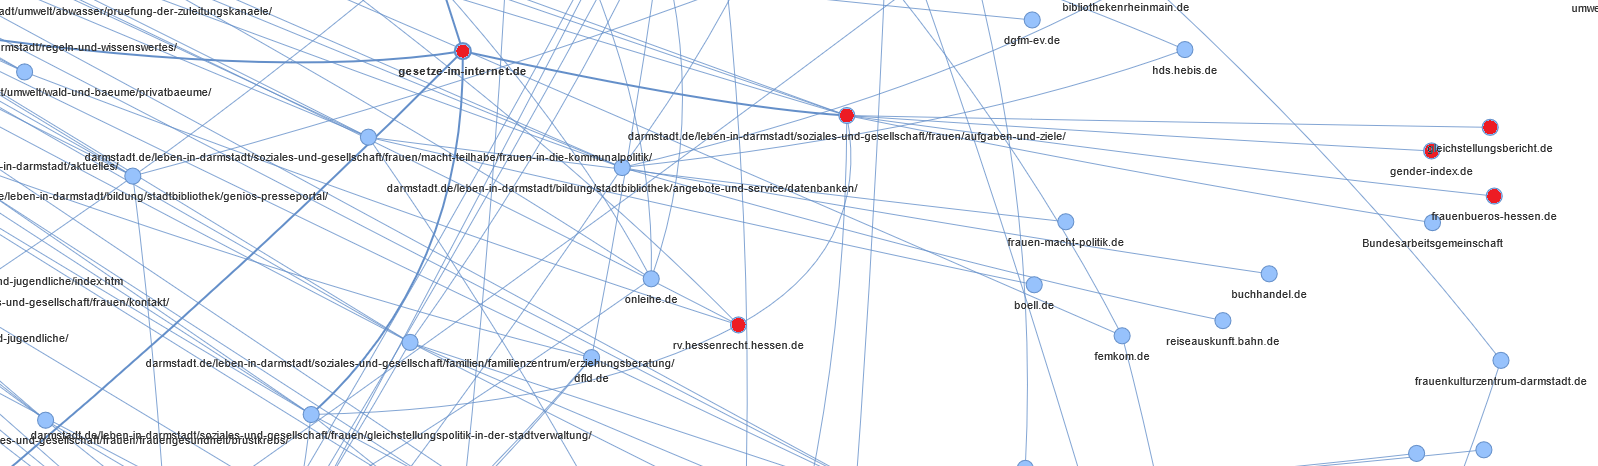
\includegraphics[width=\textwidth]{images/DarmstadtSpiderGraph2.png}

\subsection{GrapplingInsiderSpider}

Wir starteten auf der Seite \url{https://grapplinginsider.com/news}, die eine Auflistung der neusten Artikel beinhaltet und bewegten uns von dort in jeden einzelnen Artikel, sowie über den Next Button auf die nächste Seite der neusten Artikel, bis alle Artikel der Webseite gecrawled waren. Je Artikel crawlten wir URL, Kategorien, Titel, Text und Links, letztere als Ziel-URL und zugehörigem Text. \\

\noindent Siehe \texttt{GrapplingInsiderSpider.py}.

\subsection{XPath und Tupel}

{\color{MidnightBlue}
\begin{lstlisting}
categories_xpath = response.xpath("//a[@rel='category tag']")
title_xpath = response.xpath("//header/h1[@itemprop='headline']")
text_xpath = response.xpath("//div[@itemprop='articleBody']")
\end{lstlisting}}

\subsection{GrapplingInsiderSpider Analyse}

\subsubsection*{Top-Level Domains}

\begin{center}
	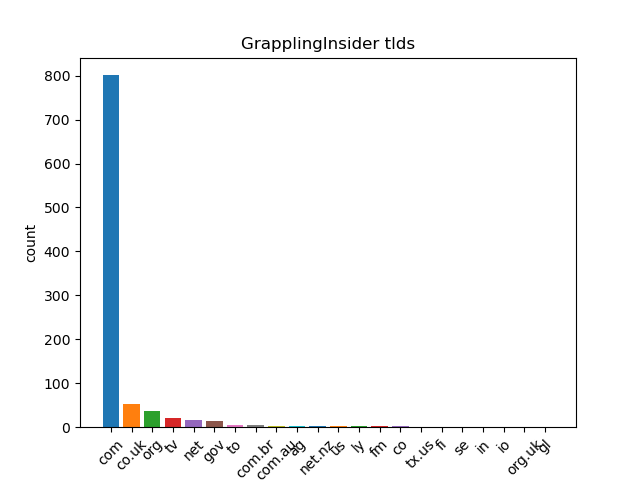
\includegraphics[width=0.66\textwidth]{images/GrapplingInsiderTLDs.png}
\end{center}

\noindent Die mit Abstand häufigste Top-Level Domain (TLD) der verlinkten Webseiten ist 'com', was bei einer amerikanischen Webseite zu erwarten war. Selten kamen weiterhin 'co.uk' als weitere englische TLD und die üblichen 'org' für Organisationen, 'tv' welche häufig für Streaming Webseiten genutzt wird, 'net' als häufige generische TLD und 'gov' für Regierungen vor. Die Verteilung ist noch stärker auf die häufigste TLD konzentriert als in den Darmstadt Daten, da die international häufige 'com' TLD hier direkt mit an Platz eins ist, statt separat neben 'de'.

\subsubsection*{Links}

Folgende ausgehenden URLs, welche von mehreren Seiten verlinkt wurden, sind uns besonders aufgefallen:

{\color{MidnightBlue}
\begin{lstlisting}
bbc.co.uk
grapplinginsider.com/uaejjf-postpones-all-bjj-events-over-coronavirus-fears/
grapplinginsider.com/coronavirus-outbreak-cancels-adcc-mongolia/
grapplinginsider.com/british-judo-black-belt-found-guilty-of-murder/
grapplinginsider.com/demi-lovato-just-got-a-stripe-on-her-blue-belt-and-its-awesome/

foxbusiness.com
grapplinginsider.com/former-nypd-detective-pushes-for-brazilian-jiu-jitsu-training-for-police/
grapplinginsider.com/love-him-or-hate-him-you-really-should-not-be-excited-to-see-president-trump-at-ufc-244/

nytimes.com
grapplinginsider.com/the-new-york-times-investigates-fight-sports-sexual-assault-allegations/
grapplinginsider.com/watch-backyard-fight-club-streetbeefs-holds-its-first-grappling-match/
grapplinginsider.com/khabib-to-mcgregor-you-are-a-rapist/

usatoday.com
grapplinginsider.com/love-him-or-hate-him-you-really-should-not-be-excited-to-see-president-trump-at-ufc-244/
grapplinginsider.com/ufc-targets-askren-maia-matchup/      

winknews.com
grapplinginsider.com/the-new-york-times-investigates-fight-sports-sexual-assault-allegations/
grapplinginsider.com/roberto-cyborg-abreu-announces-new-guidelines-to-address-misconduct-at-fight-sports/
grapplinginsider.com/roberto-cyborg-abreu-and-vagner-rocha-issue-statements-regarding-marcel-goncalves-sexual-assault-allegations/
\end{lstlisting}}

\noindent$\Rightarrow$ Diese Artikel behandeln News die es in die Mainstream Nachrichten geschafft haben.

{\color{MidnightBlue}
\begin{lstlisting}
healthline.com
grapplinginsider.com/rib-injuries-in-bjj-causes-diagnosis-and-prevention/
grapplinginsider.com/high-rollerz-bjj-and-the-cannabis-community/

ncbi.nlm.nih.gov
grapplinginsider.com/best-supplements-to-help-you-sleep-after-bjj/
grapplinginsider.com/focus-on-sleep-not-supplements/
grapplinginsider.com/bjj-low-testosterone-test-lets-get-checked/
\end{lstlisting}}

\noindent$\Rightarrow$ Diese Artikel behandeln Gesundheit und Medizin.

{\color{MidnightBlue}
\begin{lstlisting}
mginaction.com
grapplinginsider.com/marcelo-garcia-set-to-release-butterfly-guard-instructional/
grapplinginsider.com/5-reasons-why-marcelo-garcia-is-the-greatest-of-all-time/
\end{lstlisting}}

\noindent$\Rightarrow$ Diese Artikel behandeln einen bekannten Wettkämpfer und verweisen auf dessen Webseite.

\newpage
\subsubsection*{Weitere Analyse}

Auch hier entschieden wir uns wieder für eine Graphrepräsentation mittels \texttt{networkx} und \texttt{pyvis}.

\begin{center}
	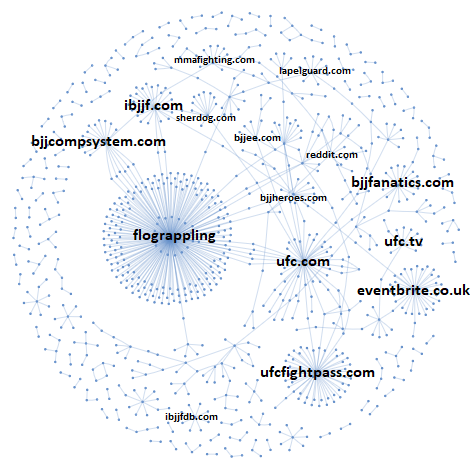
\includegraphics[width=0.5\textwidth]{images/GrapplingInsiderGraph.png}
\end{center}

\noindent Hier sieht man klare Cluster von Artikeln um Webseiten gro{\ss}er, bekannter Organisationen. Die grö{\ss}ten sind die Webseiten die Events streamen (\texttt{flograppling}, \texttt{ufc}), die gro{\ss}en Veranstalter und Veranstaltungsaggregatoren (\texttt{ufc}, \texttt{ibjjf}, \texttt{eventbrite}), \texttt{bjjfanatics} welche Lehrvideos verkauft, Foren (\texttt{sherdog}, \texttt{reddit}) und weitere News Webseiten (\texttt{bjjheroes}, \texttt{bjjee}, \texttt{mmafighting}).